\section{Anhang}

%Fluoreszenzintensität von DPPC als Funktion der Temperatur 
\begin{figure}[h!]
	\begin{center}
		\begin{minipage}{0,8\textwidth}
			
			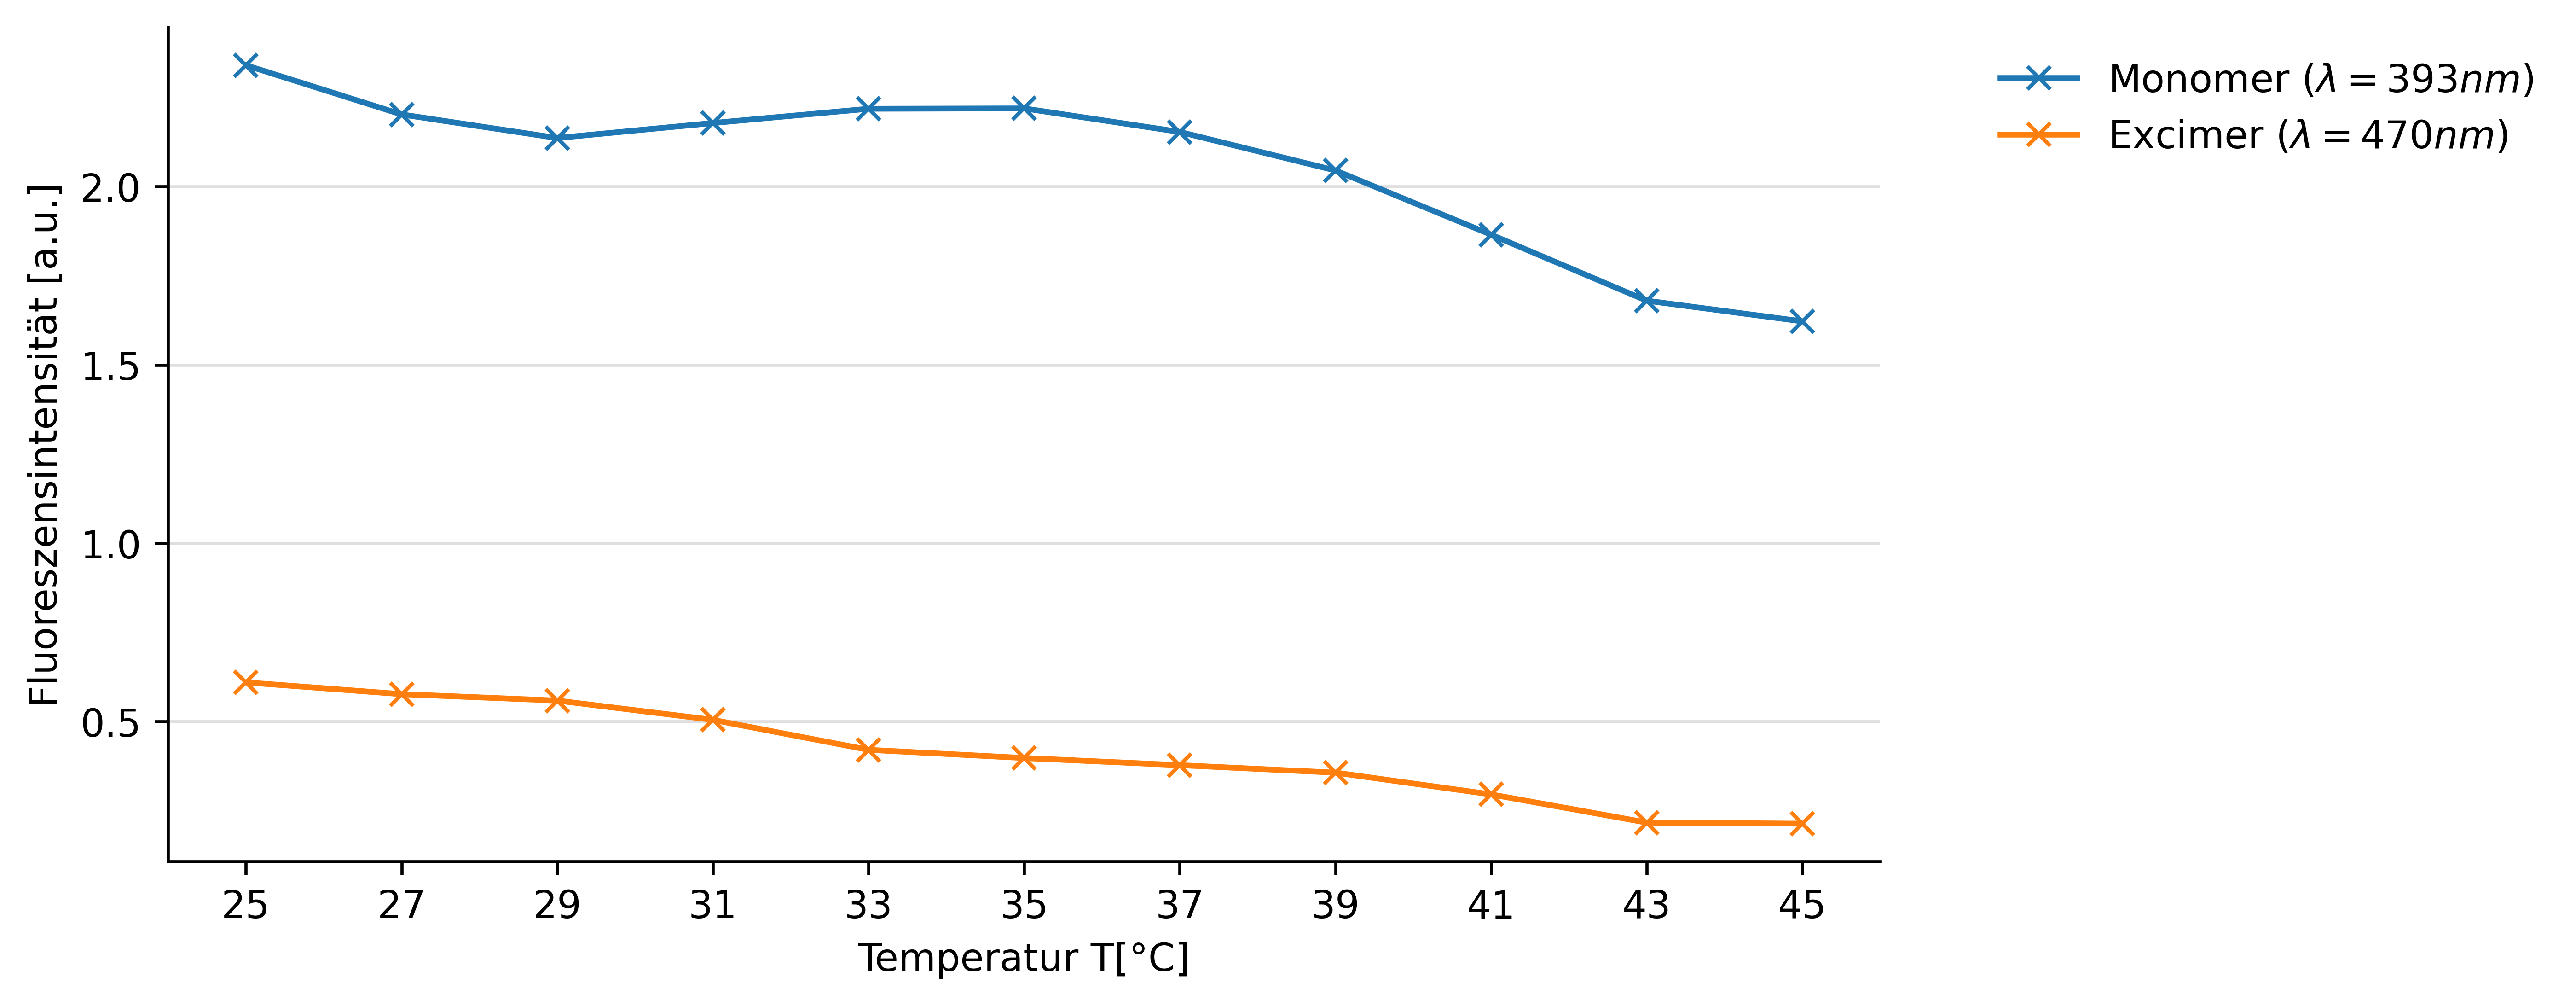
\includegraphics[width=\textwidth]{analysis/reports/DPPC_Temp.png}
			\caption{Pyren in DPPC Vesikeln; Fluoreszenzintensität als Funktion der Temperatur} 
			\label{Monomer_Temp} 
		\end{minipage}
	\end{center}
\end{figure}

%Fluoreszenzintensität von Ei-PC als Funktion der Temperatur 
\begin{figure}[h!]
	\begin{center}
		\begin{minipage}{0,8\textwidth}
			
			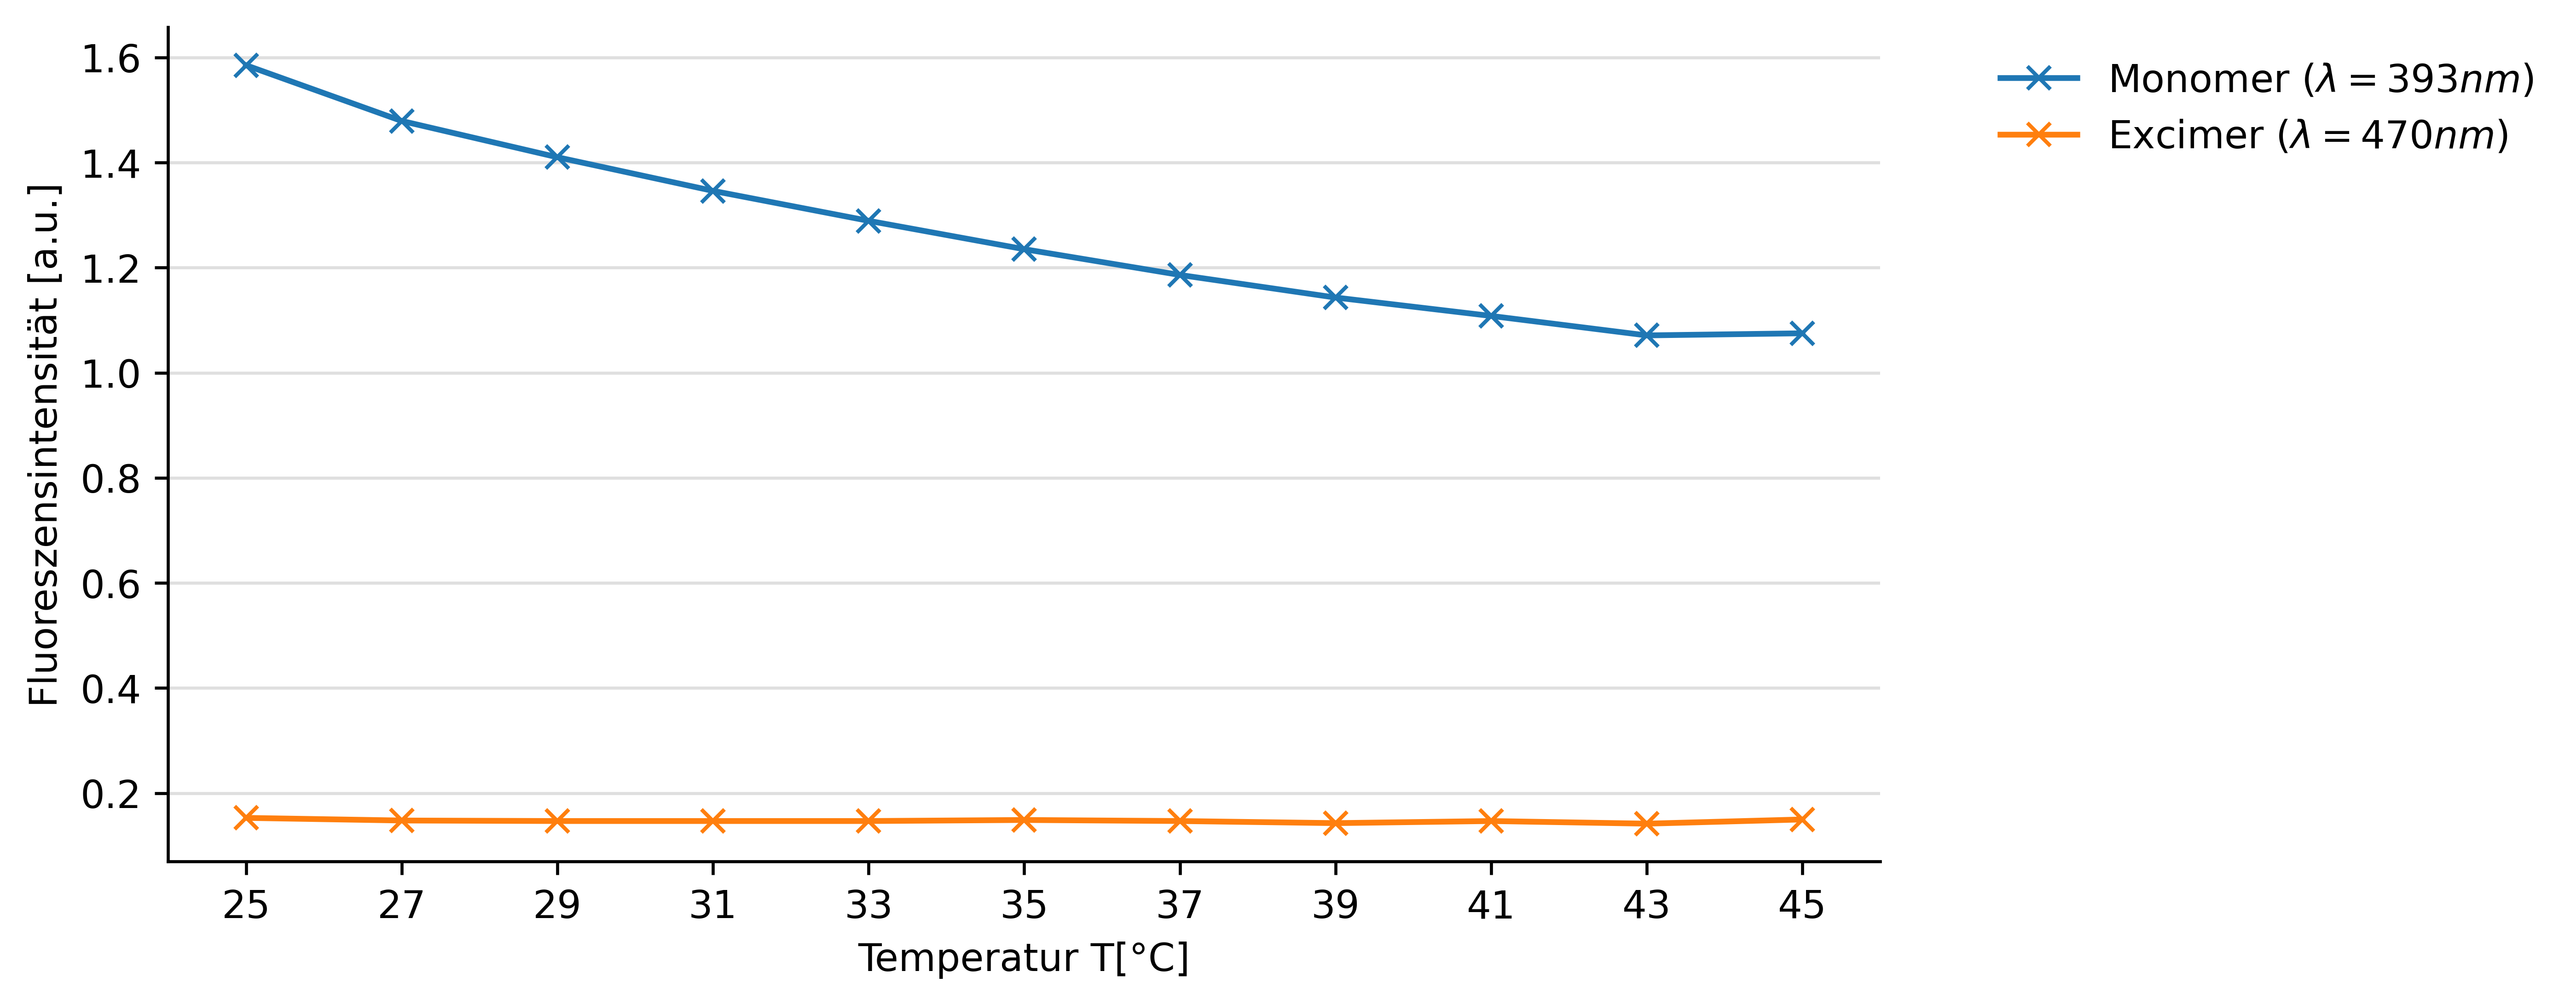
\includegraphics[width=\textwidth]{analysis/reports//Ei-PC_Temp.png}
			\caption{Pyren in Ei-PC Vesikeln; Fluoreszenzintensität als Funktion der Temperatur} 
			\label{Excimer_Temp} 
		\end{minipage}
	\end{center}
\end{figure}
